In this section we use visualization method in order to explore the distribution of the independent data variables and thier relationships with the turn taking (which is the depended variable)
%
The visualization was done using python seaborn library which is based on matplotlib. The data set for the visualization contains a row for each dialog act. For each dialog act we measure its length, and the values of the summary features (RTL and RTC). The independent variable denote wether a turn change occured after the dialog act.

\begin{table}[ht!]
\begin{center}
\begin{tabular}{llllrr}
\toprule
Variable &  Description & Type &\\
\midrule
     Previous Dialog Act & the dialog act before the current one  & categorical\\
     Dialog Act & the current dialog act & categorical \\
     Length & length of the current dialog act in seconds & seconds \\
     Relative Turn Length (RTL)  & Relative turn length as defined in \ref{sfeatures} & percent \\
     Relative Time Control (RTC) & Relative time control as defined in \ref{sfeatures} & percent \\
     Turn Change & 1 if there was a turn change after this dialog act & binary \\
\bottomrule
\end{tabular}
\end{center}
\caption{Data Fields}
\end{table}


\subsection{Dialog Acts}

The first visualization, Figure \ref{f1} plots the distribution of each dialog act in the corpus. Each bar is a count of the dialog act type, divided by the total dialog acts.  We can observe that the majority of dialog acts are statements, backchannels and opinions. This is true to the nature of the switchboard corpus which consists mainly of casual conversations.

 \begin{figure}[ht!]
 \centering
 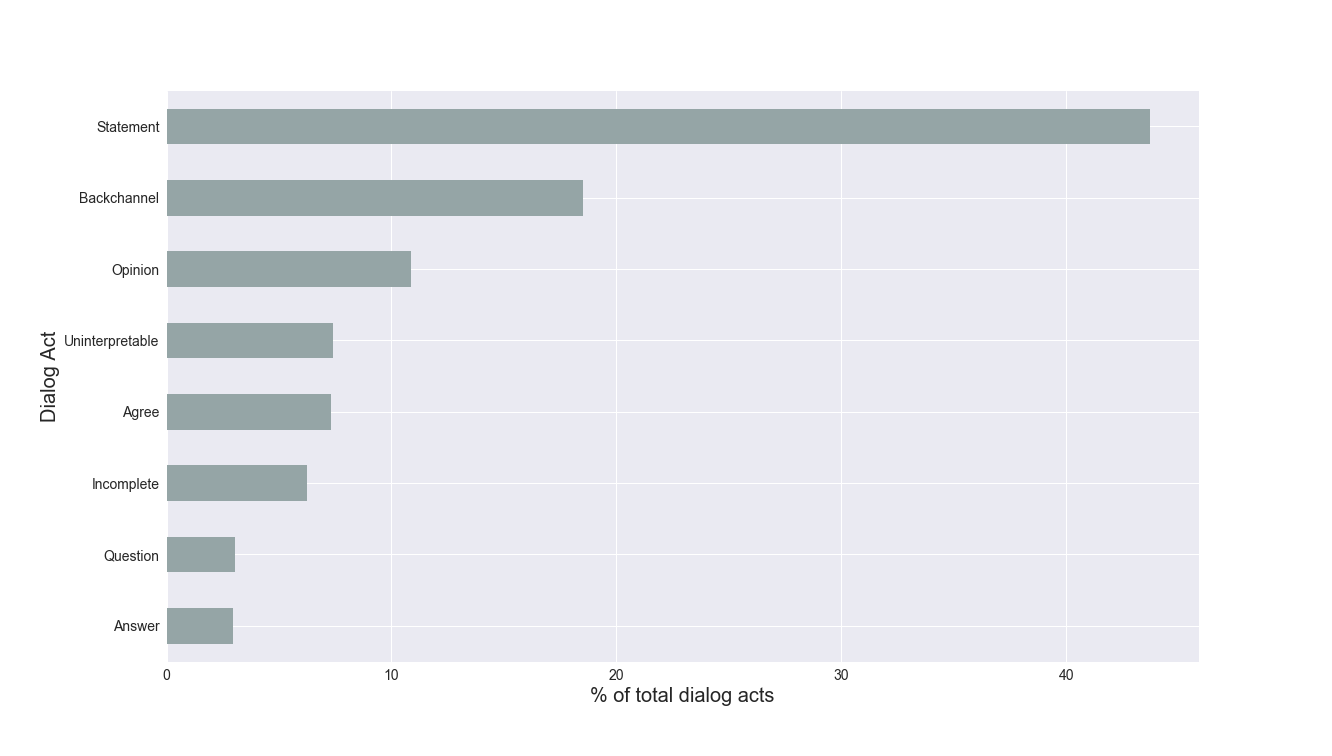
\includegraphics[width=\textwidth]{../scikitlearn/figures/f1.png}
 \caption{Dialog act relative count\label{overflow}}
 \label{f1}
 \end{figure}

Next we wanted to measure the correlation between dialog act type and the probability of a turn change.  In figure \ref{f2}, each bar measures the number of time a turn change occurred after a dialog act type divided by the total dialog act of this type. Or the probability that a dialog act of the said type will lead to turn change. We observe that the majority of back channels and question (which are usually the first utterance in an question-answer adjacency pair) will lead to a turn change.

\begin{figure}[ht!]
\centering
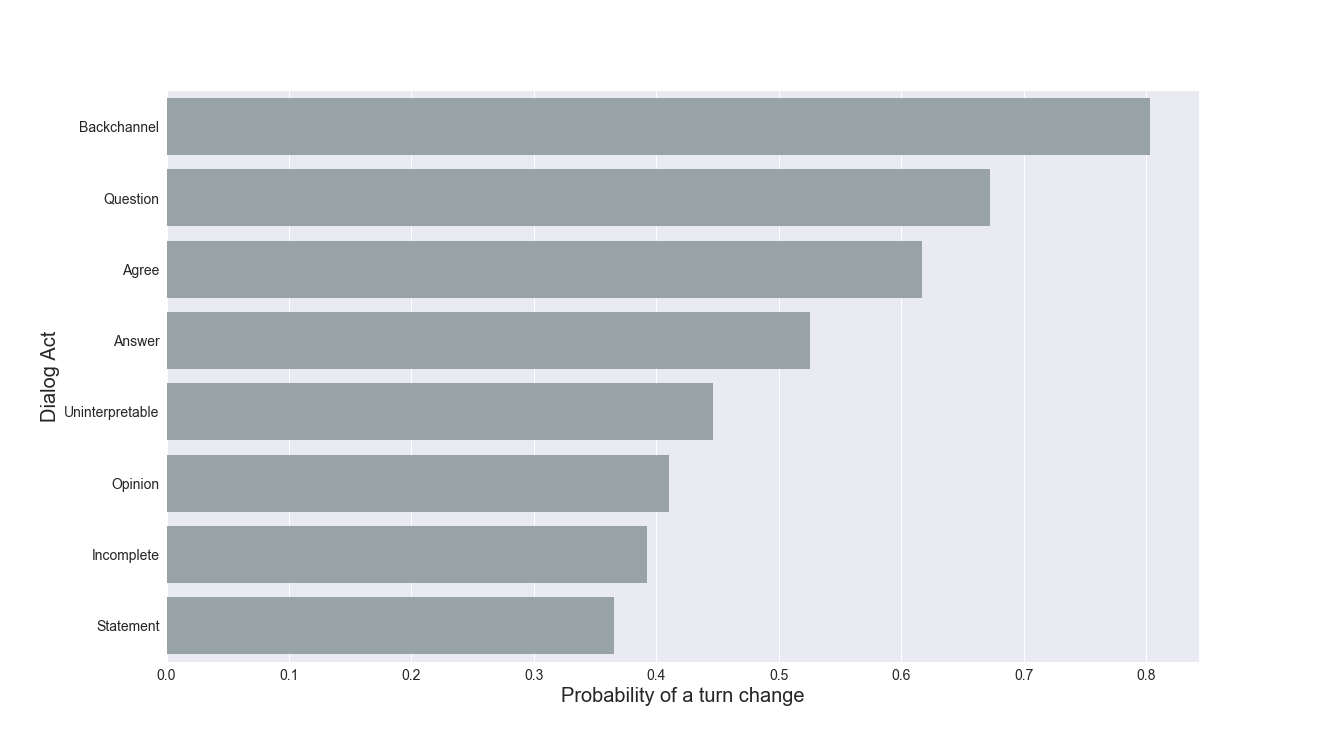
\includegraphics[width=\textwidth]{../scikitlearn/figures/f2.png}
\caption{Dialog act probability of turn change\label{overflow}}
\label{f2}
\end{figure}

Next we measured the the relative turn length score for each type of dialog act.
In \ref{f3}, for each dialog act we show the distribution of relative turn length score for act that
led to turn change and act that did not. We can see that in most of the dialog acts,
the median RTL score that led to turn change is smaller than RTL score of acts of which
the speaker kept the floor. This suggests that a speaker which uses the floor more than its
avarage turn length will tend to hold the floor even more.
 

\begin{figure}[ht!]
\centering
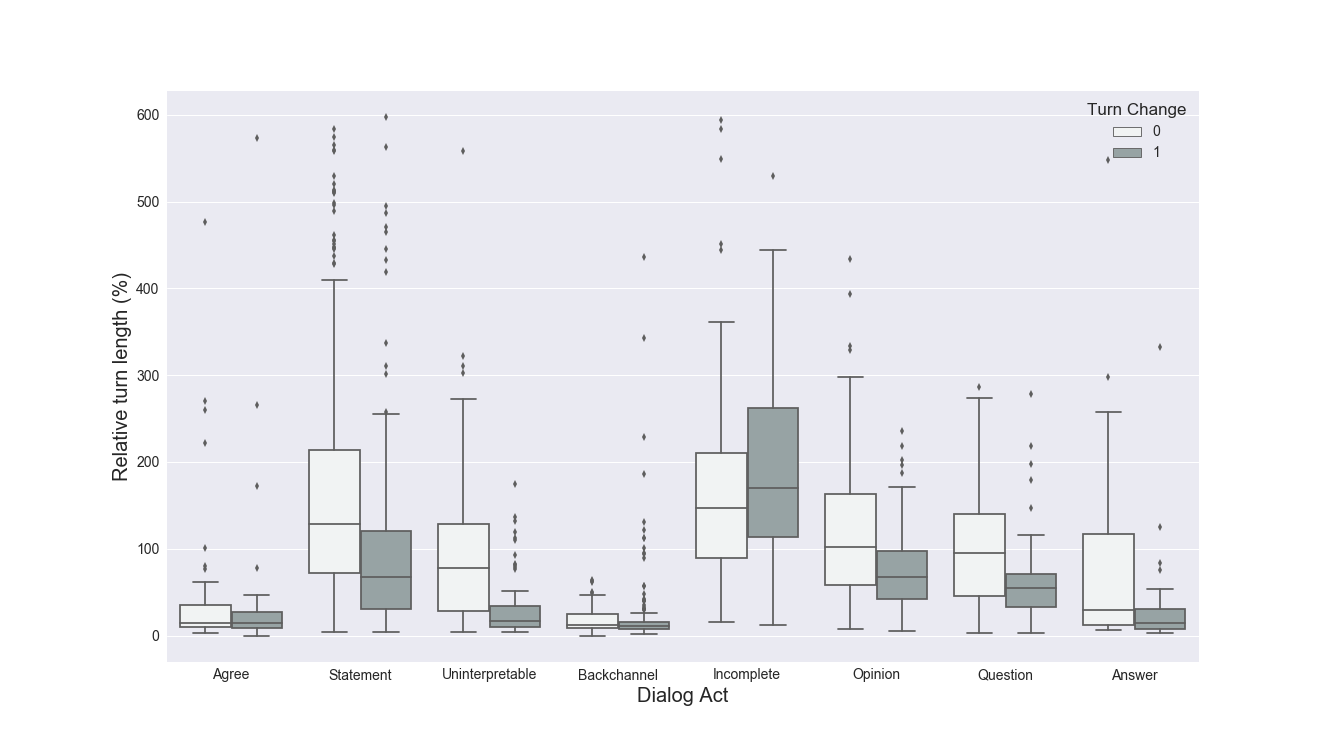
\includegraphics[width=\textwidth]{../scikitlearn/figures/f3.png}
\caption{RTL score for dialog act type\label{overflow}}
\label{f3}
\end{figure}

Next we measured the relative floor control score for each type of dialog act.
In \ref{f4}, for each dialog act we show the distribution of relative floor control for act that
led to turn change and act that did not. We can see that in most of the dialog acts,
the median score is about equal and close to 50\%. We can observe that for the question dialog act, when the speaker had high relative floor control, it tend to keep the turn after the question (for example, by asking rhetorical question) 

\begin{figure}[ht!]
\centering
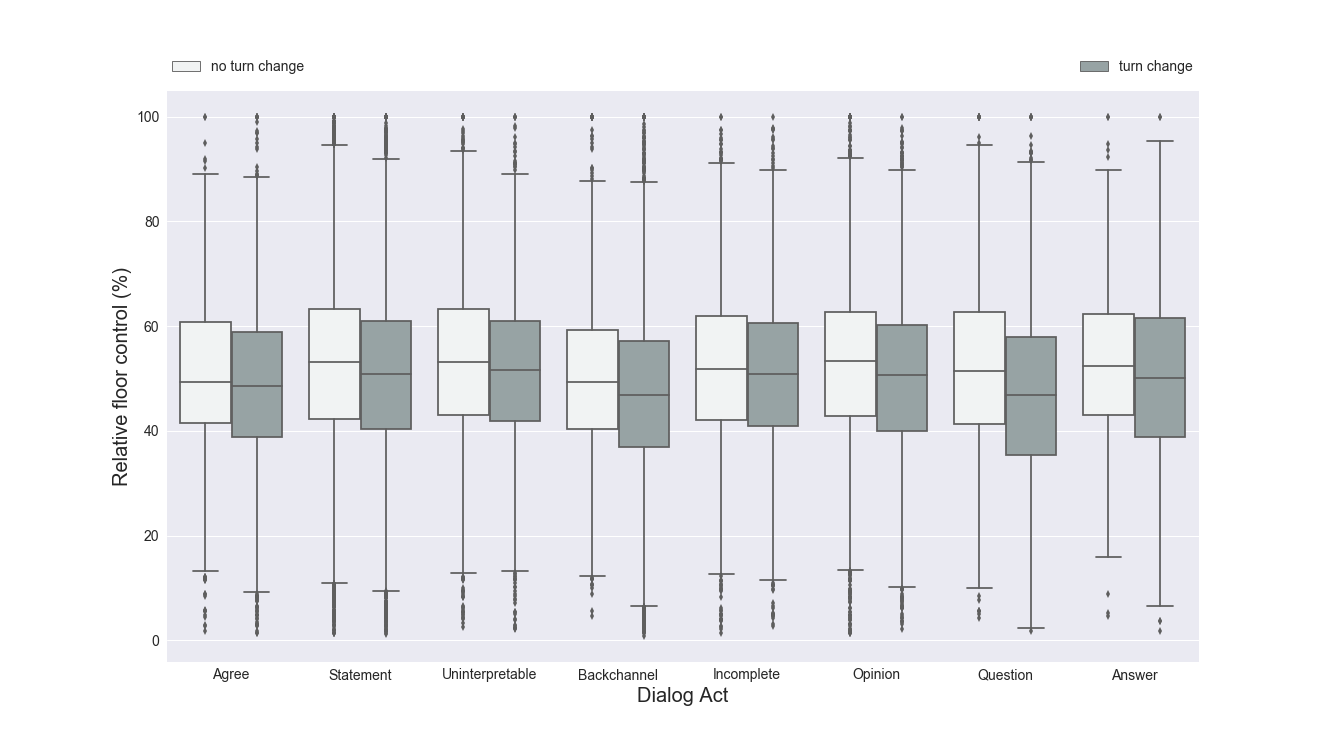
\includegraphics[width=\textwidth]{../scikitlearn/figures/f4.png}
\caption{Dialog act probability of turn change\label{overflow}}
\label{f4}
\end{figure}

Next we measured the relation between values of relative turn length and probability of turn change. 
To compute figure \ref{f4}, we divided the range of relative floor control into buckets and counted for each bucket the number of dialog acts (regardless of the type) that led to a turn change and the total dialog acts in the bucket.
We than computed the probability of a turn change by dividing the former by the latter. As shown, when the chance of turn transfer is higher when the speaker has the floor for the relative short amount of a time ( probably the affect of back channel). We can also observe that as the speaker has the floor for more time, it tend to hold it.


\begin{figure}[ht!]
\centering
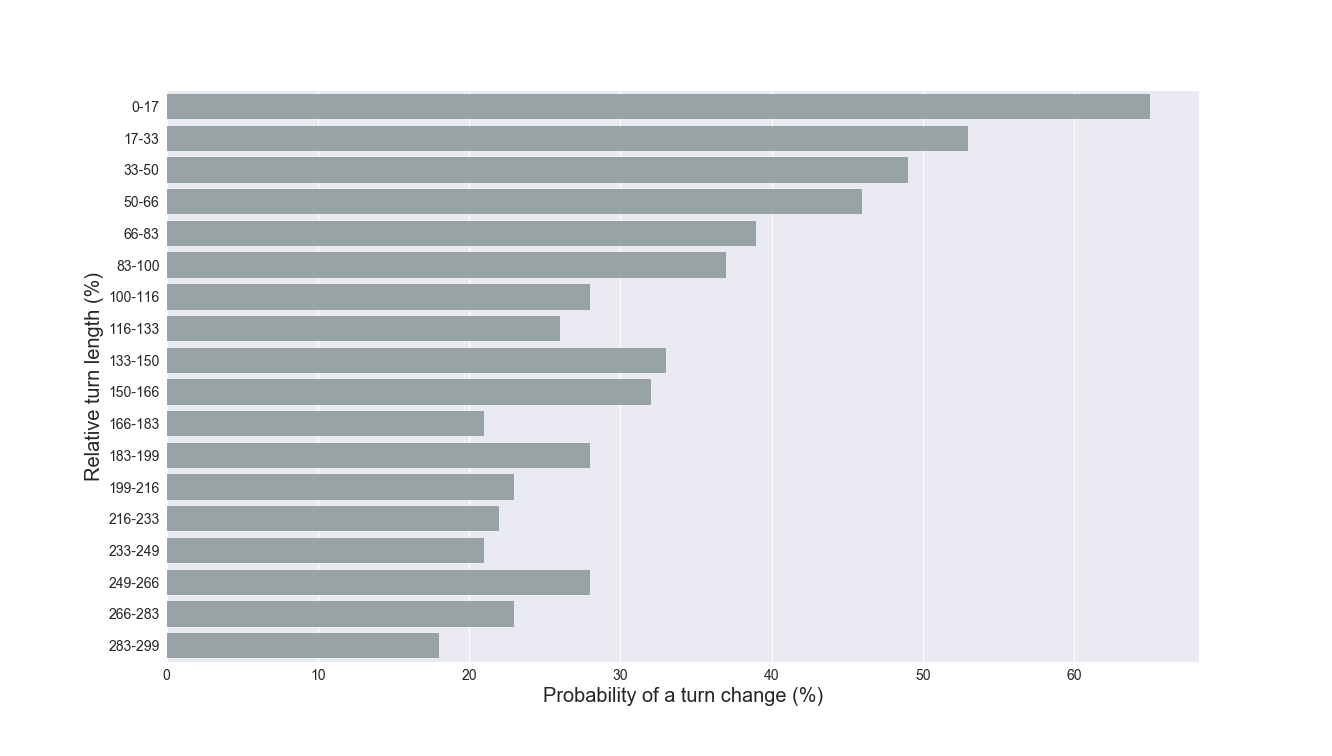
\includegraphics[width=\textwidth]{../scikitlearn/figures/f5.png}
\caption{Relative floor control affect on probability of a turn change\label{overflow}}
\label{f4}
\end{figure}

Next we measured the relation between values of relative floor control and probability of turn change.
As with relative turn length, to compute figure \ref{f4}, we divided the range of relative floor control into buckets and counted for each bucket the number of dialog acts (regardless of the type) that led to a turn change and the total dialog acts in the bucket.
Again, we than computed the probability of a turn change by dividing the former by the latter. As shown, 
we can see that the relative floor control does not have a lot of affect on the proababilty of a turn change. However, we can notice that when the speaker has relative floor control scores above 50\% it tend to keep the floor and avoid turn change.

\begin{figure}[ht!]
\centering
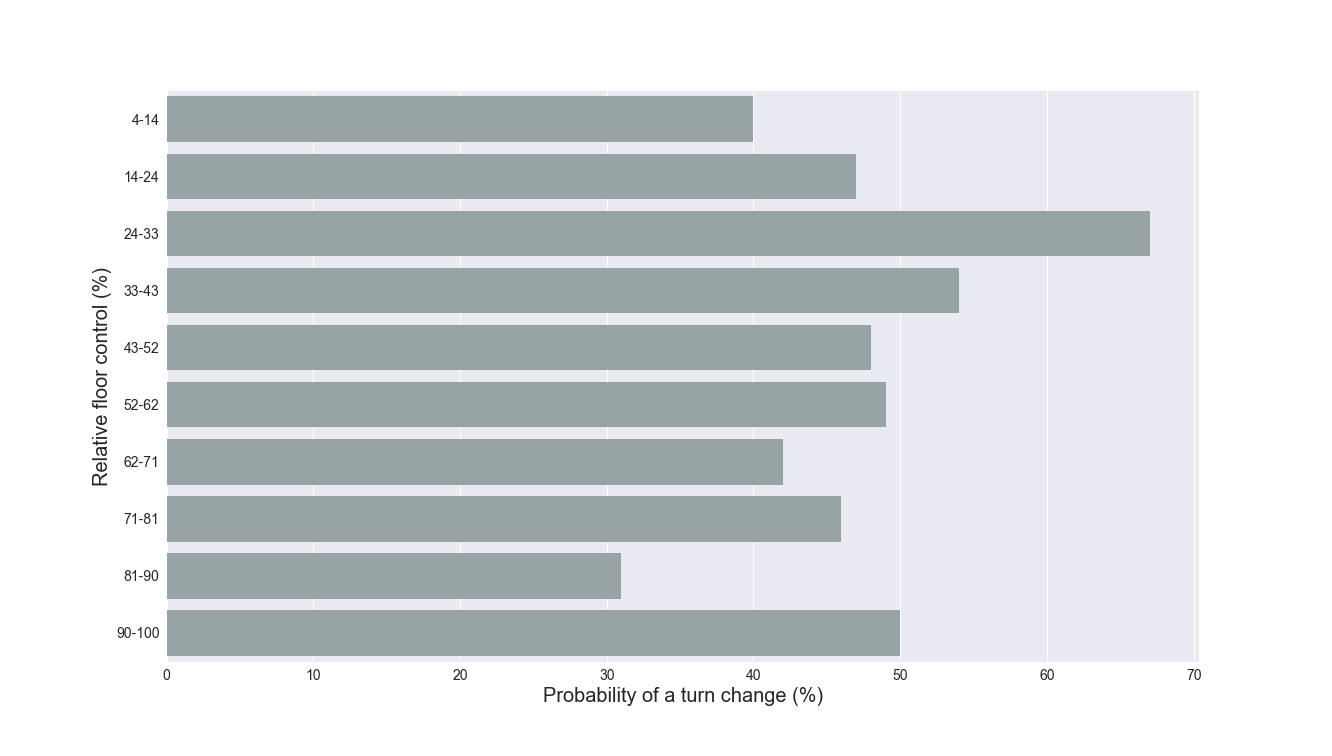
\includegraphics[width=\textwidth]{../scikitlearn/figures/f6.png}
\caption{Dialog act probability of turn change\label{overflow}}
\label{f4}
\end{figure}
